En este trabajo práctico vamos a analizar el camino que recorre un datagrama IP para llegar a un destino en particular. El protocolo TCP/IP posee un módulo llamado ICMP para los mensajes de control y de error.
En nuestro caso el origen de los paquetes será el Gran Buenos Aires y mientras que los destinos serán universidades de distintos países del mundo. Para ver el camino que transitan los paquetes que enviamos hay una herramienta llamada \emph{traceroute}, la cual indica el camino y cuanto fue el round trip time.
Nosotros codificamos nuestra propia versión de traceroute y realizamos nuestros experimentos con ella.

\subsection{Experimentos}
\par Al enviar un paquete con un host de destino, este es redireccionado por distintos hosts (a los que llamaremos \textit{nodos}) que lo conducen hacia el destino. Al recibir un paquete, un nodo realiza los siguientes pasos (entre otros):
\begin{enumerate}
  \item revisa el destino: si es él lo toma y no ejecuta ninguno de los otros pasos.
  \item revisa el campo \textit{ttl}\footnote{Este campo indica la cantidad de nodos por los cuales puede continuar el paquete. Si este valor llega a cero se debe devolver un paquete al origen con el tipo \textit{time exceded}.}: si es cero, crea un paquete de tipo \textit{time exceded} y se lo envía al host de origen y no ejecuta ninguno de los otros pasos.
  \item envía el paquete al siguiente nodo: dependiendo de su tabla de forwarding y configuración selecciona el nodo al cual le envía el paquete para que continúe su camino al destino.
\end{enumerate}
\begin{figure}[ht]
  \begin{subfigure}[b]{.5\textwidth}
    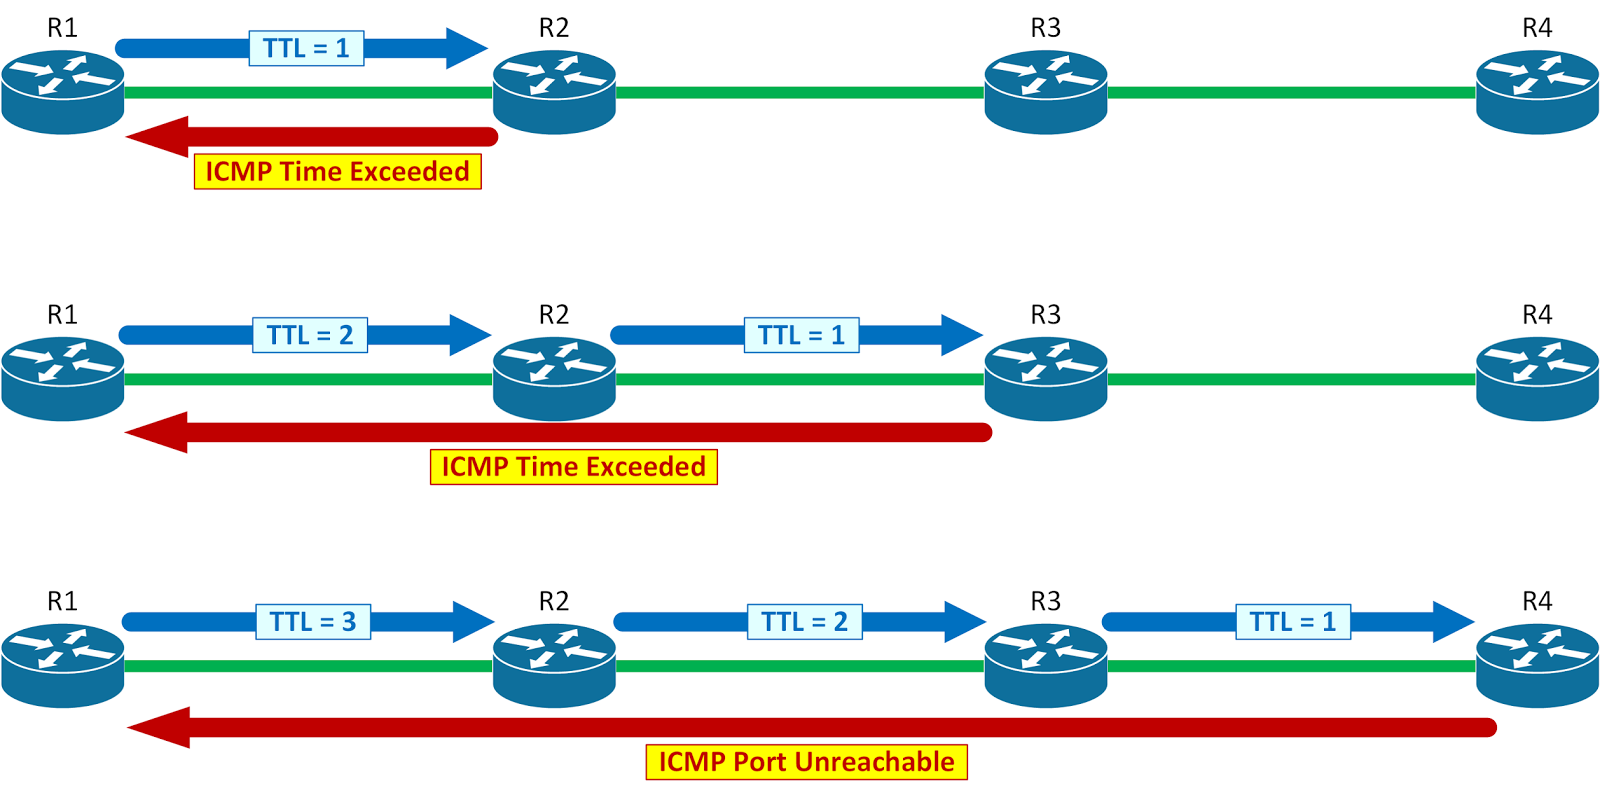
\includegraphics[width=\textwidth]{Imagenes/explicacion_traceroute.png}
  \end{subfigure}
  \label{fig:explicacion_traceroute}
  \caption{Ejemplo de ejecución de nuestro algoritmo para detectar la ruta desde R1 hasta R4}
\end{figure}
\par Nos proponemos analizar los caminos por los cuales distintos paquetes llegan al destino. Para esto usaremos mensajes de protocolo ICMP, donde iremos aumentando el campo \textit{ttl} y provocaremos así que los nodos nos contesten con mensajes del tipo \textit{time exceded}. Controlaremos el tiempo que tarda cada nodo en contestar (\textit{rtt}) por si un hop no responde y luego analizaremos esos valores en busca de saltos intercontinentales.

\par Para determinar si un salto entre dos nodos es intercontinental nos basaremos en la técnica de estimación de outliers propuesta por Cimbala\footnote{http://www.mne.psu.edu/cimbala/me345/Lectures/Outliers.pdf}. Identificaremos outliers y trabajaremos con ellos para determinar si son saltos intercontinentales.
Cimbala propone una métrica basada en un z-score para cada uno de los RTT promedio de cada uno de los hops, el cual está definido de la siguiente manera:

\begin{equation}
    ZRTT_i = \frac{RTT_i-mean(RTT)}{std(RTT)}
\end{equation}
donde $mean(RTT)$ es la media aritmética de los RTTs de la ruta y $std(RTT)$ el desvío estándar.
Luego al mayor de estos valores se lo debe comparar con un valor crítico dado por la siguiente ecuación:

\begin{equation}
    \tau = \frac{t_{\alpha/2}*(n-1)}{\sqrt{n}*\sqrt{n-2+t_{\alpha/2}^{2}}}
\end{equation}
donde $n$ es la cantidad de hops y $t_{\alpha/2}$ es la distribución de student con el parámetro $\alpha=0.05$ y $df =  n-2$
Si $ZRRT_{max} > \tau$ se considera que que esa medición es un outlier y se lo separa de la muestra para luego repetir el proceso desde el cálculo de los ZRTTs
\par Al mismo tiempo, utilizaremos un servicio de api externo\footnote{https://github.com/fiorix/freegeoip} para obtener la geolocalización de cada nodo (por medio de la ip). De esta manera podremos seguir el recorrido del paquete hacia el destino y verificar el funcionamiento del método utilizado para detectar saltos intercontinentales. Para las funciones relativas al manejo de paquetes usamos una biblioteca de Python llamada \emph{Scapy}
